\chapter{Implementazione}
\label{ch:Progettazione}

\section{Diagrammi di deployment}

\begin{center}
  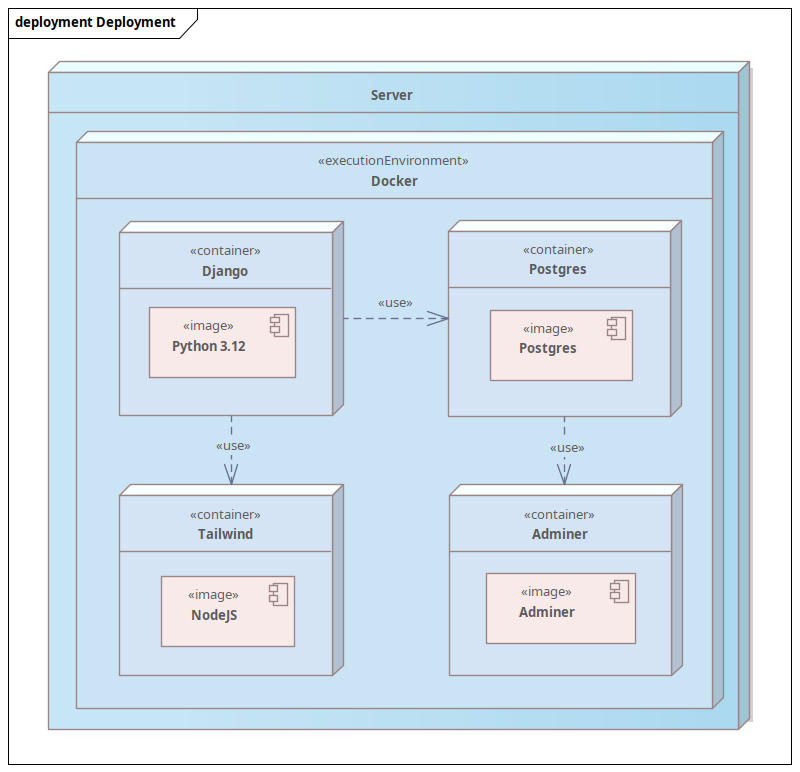
\includegraphics[width=\textwidth]{immagini/Implementazione/Deployment.png}
\end{center}

\clearpage

\section{Tecnologie utilizzate}

\subsection{Tecnologie Front-End}
\subsubsection{Django Template Language}
Django fornisce un linguaggio efficace per la realizzazione del livello front-end dell'applicazione. Questo linguaggio consente di iniettare i dati ricevuti dalla logica di backend, facilitando la generazione dinamica di contenuti.

\subsubsection{Tailwind CSS}
Tailwind CSS è un framework CSS basato su classi predefinite, progettato per costruire e progettare pagine web direttamente nel markup HTML. Il suo utilizzo ha permesso di integrare codice CSS all’interno dell’HTML, velocizzando il processo di styling del sito web grazie alla disponibilità di classi pronte all'uso.

\subsubsection{HTMX}
HTMX è una libreria JavaScript leggera e intuitiva che consente di arricchire le pagine web esistenti con funzionalità di aggiornamento dinamico e interattività. Grazie al suo utilizzo, è stato possibile creare esperienze utente interattive senza introdurre un'eccessiva quantità di codice JavaScript, preservando le performance del sistema.

\subsection{Tecnologie Back-End}
\subsubsection{Django}
Django è un web framework di alto livello, scritto in Python, che facilita lo sviluppo di siti web. È stato scelto per i suoi numerosi vantaggi rispetto ad altre tecnologie, tra cui velocità di sviluppo, sicurezza e scalabilità.

\subsubsection{PostgreSQL}
PostgreSQL è un sistema di gestione di database open source di livello aziendale. Supporta tipi di dati avanzati e offre funzionalità di ottimizzazione delle prestazioni solitamente disponibili solo in database commerciali. Il progetto utilizza PostgreSQL come DBMS.

\subsubsection{Adminer}
Adminer è uno strumento di gestione dei database che consente di creare e gestire database e tabelle, importare ed esportare dati e inviare query SQL. Nel progetto è stato utilizzato insieme a PostgreSQL per semplificare la gestione del database.

\subsection{Tecnologie Cloud}
\subsubsection{Docker}
Docker è una piattaforma open source per lo sviluppo e l'esecuzione di applicazioni in ambienti virtualizzati, detti container. Ogni microservizio del progetto è stato virtualizzato in un container, consentendo una gestione indipendente e modulare.

\subsubsection{Docker Compose}
Docker Compose è uno strumento che permette di orchestrare e gestire facilmente l'esecuzione di più container Docker. È stato utilizzato per coordinare tutti i microservizi del progetto.

\subsection{Tecnologie Version Control System}
\subsubsection{Git}
Git è un sistema di controllo di versione che consente di monitorare le modifiche apportate ai file di progetto nel tempo. Grazie a Git, è stato possibile suddividere il carico di lavoro tra i membri del team, favorendo lo sviluppo simultaneo delle funzionalità del progetto.

\subsection{Github}
GitHub è una piattaforma di hosting per progetti software che utilizza il sistema di controllo di versione distribuito Git. È stato impiegato per facilitare lo sviluppo parallelo delle funzionalità del progetto, garantendo la sincronizzazione continua del codice e fornendo un backup sicuro e centralizzato.

\subsection{Altre tecnologie utilizzate}
\subsubsection{Enterprise Architect}
Enterprise Architect è uno strumento di modellazione e progettazione visiva basato su OMG UML. Nel progetto è stato utilizzato per modellare l'architettura del sito web e supportare l'implementazione dei modelli durante l'intero ciclo di vita dello sviluppo dell'applicazione.


\clearpage
\section{Mockup}

\begin{figure}[h!]
\centering
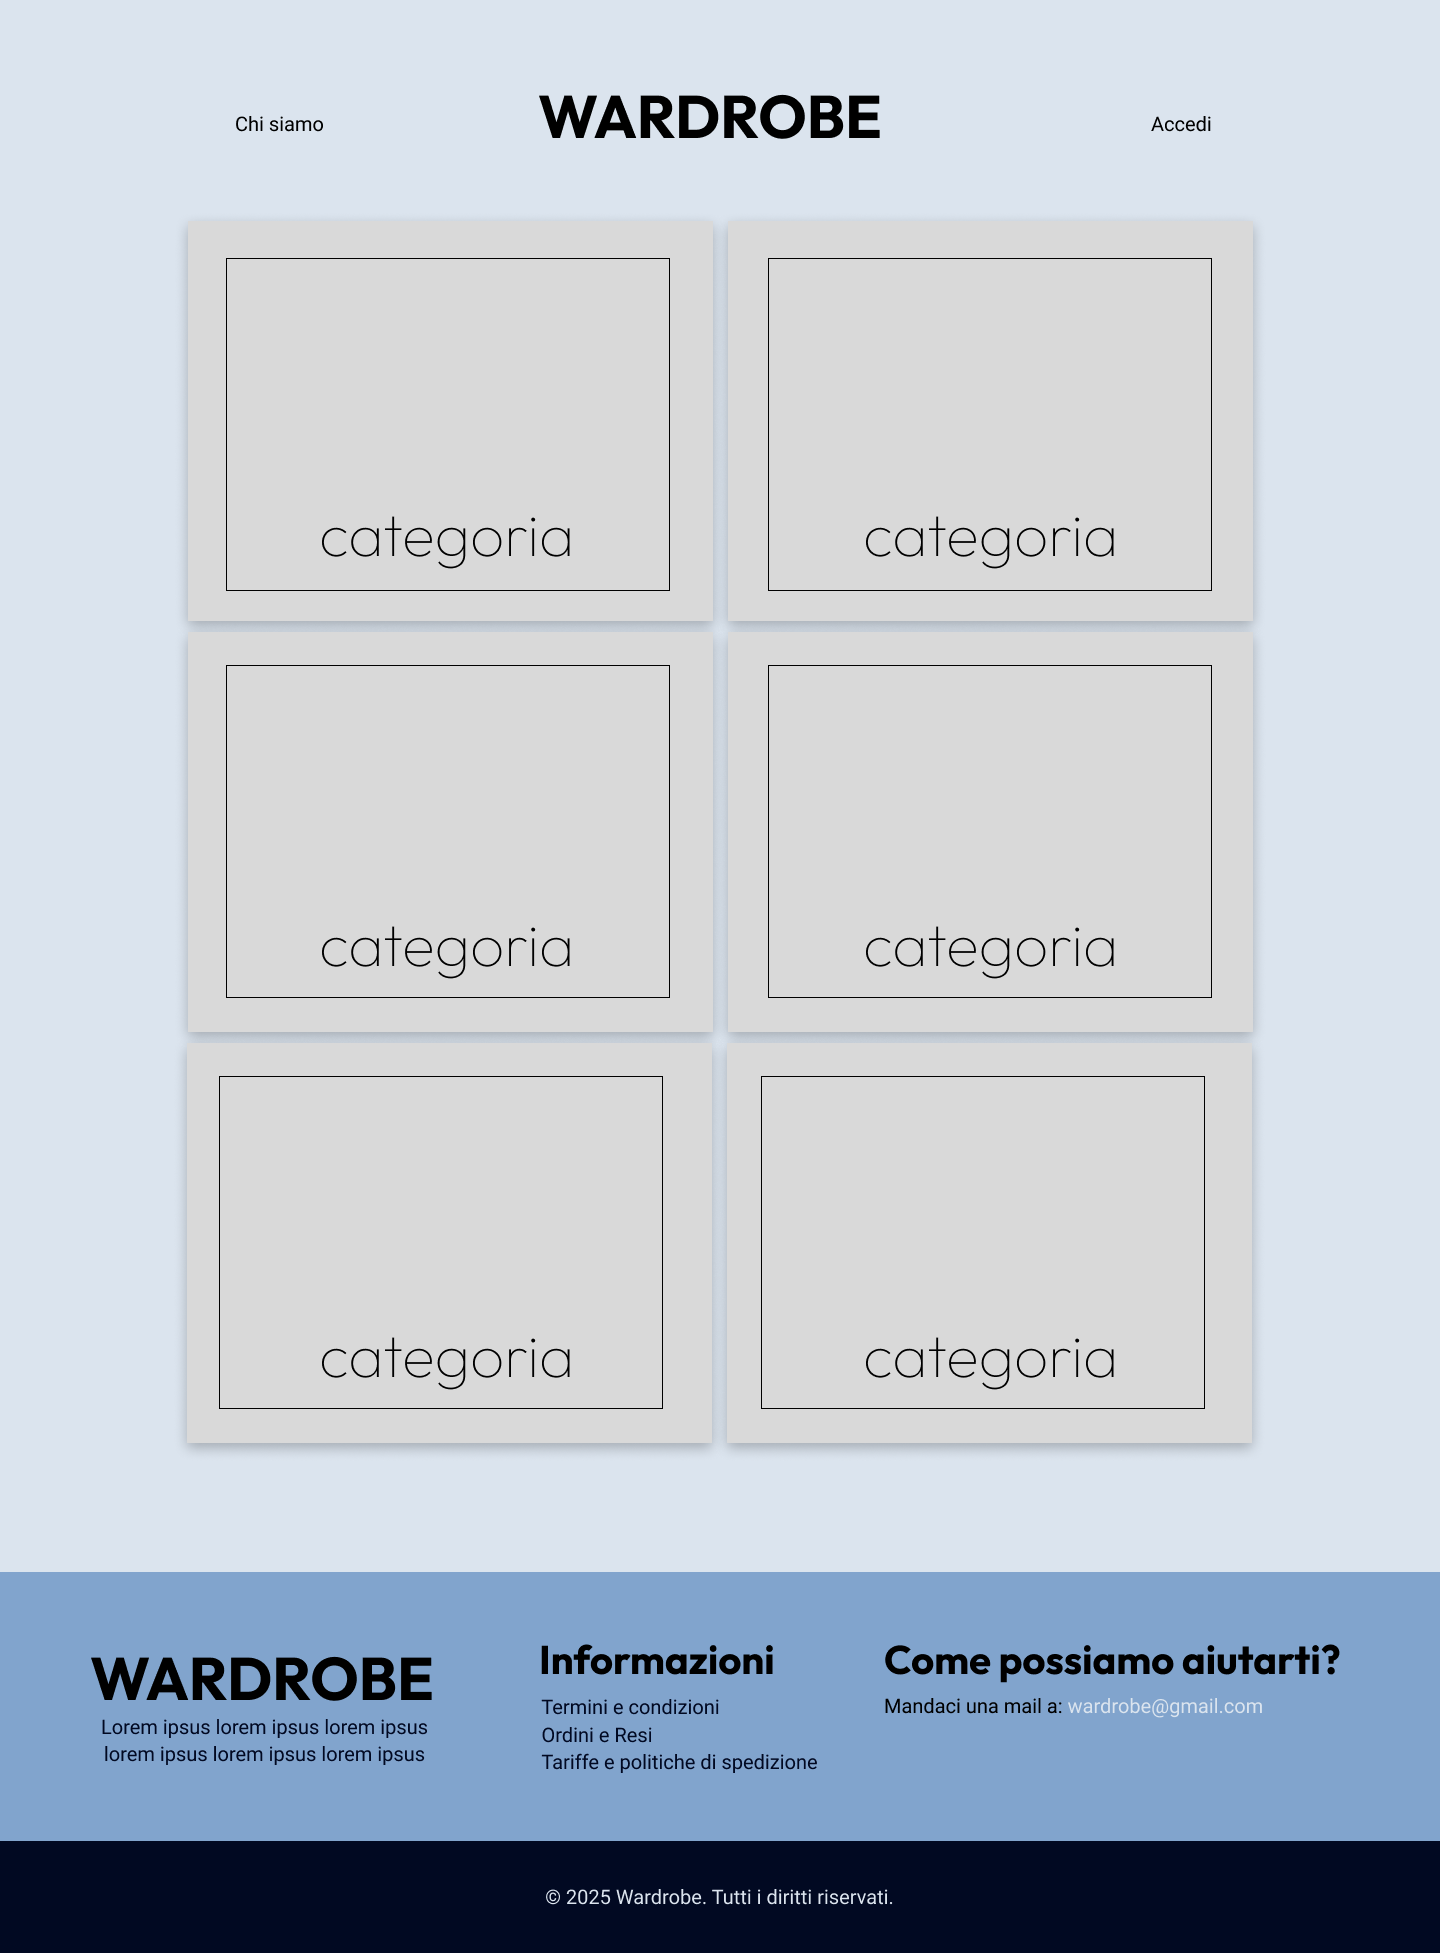
\includegraphics[width=0.8\textwidth]{immagini/Mockups/homepage.png}
\caption{Homepage}
\end{figure}

\clearpage

\begin{figure}[h!]
\centering
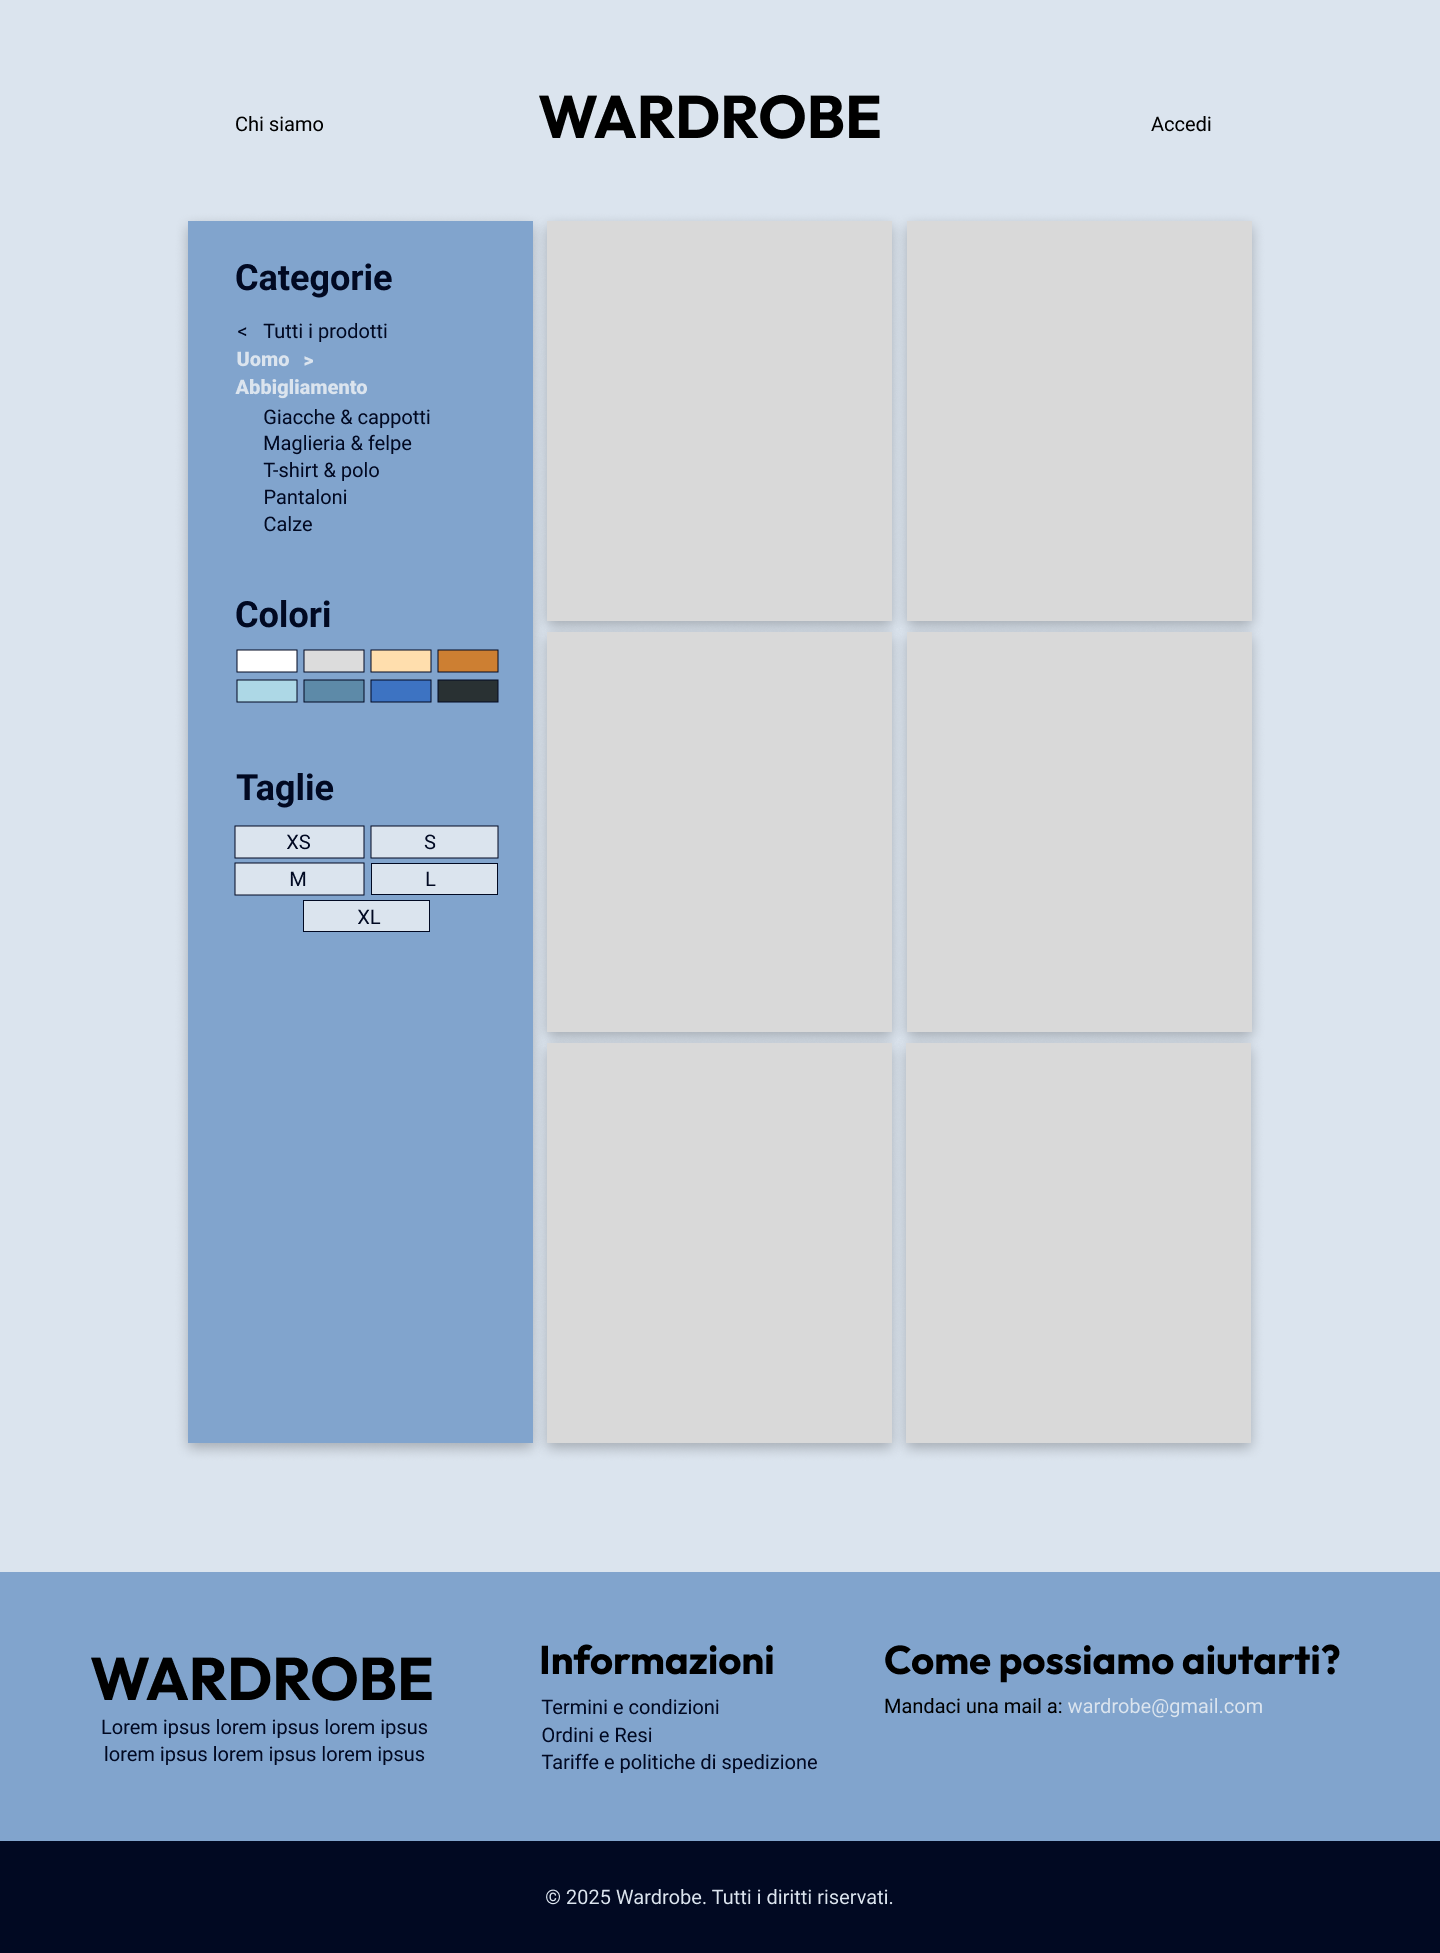
\includegraphics[width=0.8\textwidth]{immagini/Mockups/ricerca.png}
\caption{Pagina di ricerca dei prodotti}
\end{figure}

\clearpage

\begin{figure}[h!]
\centering
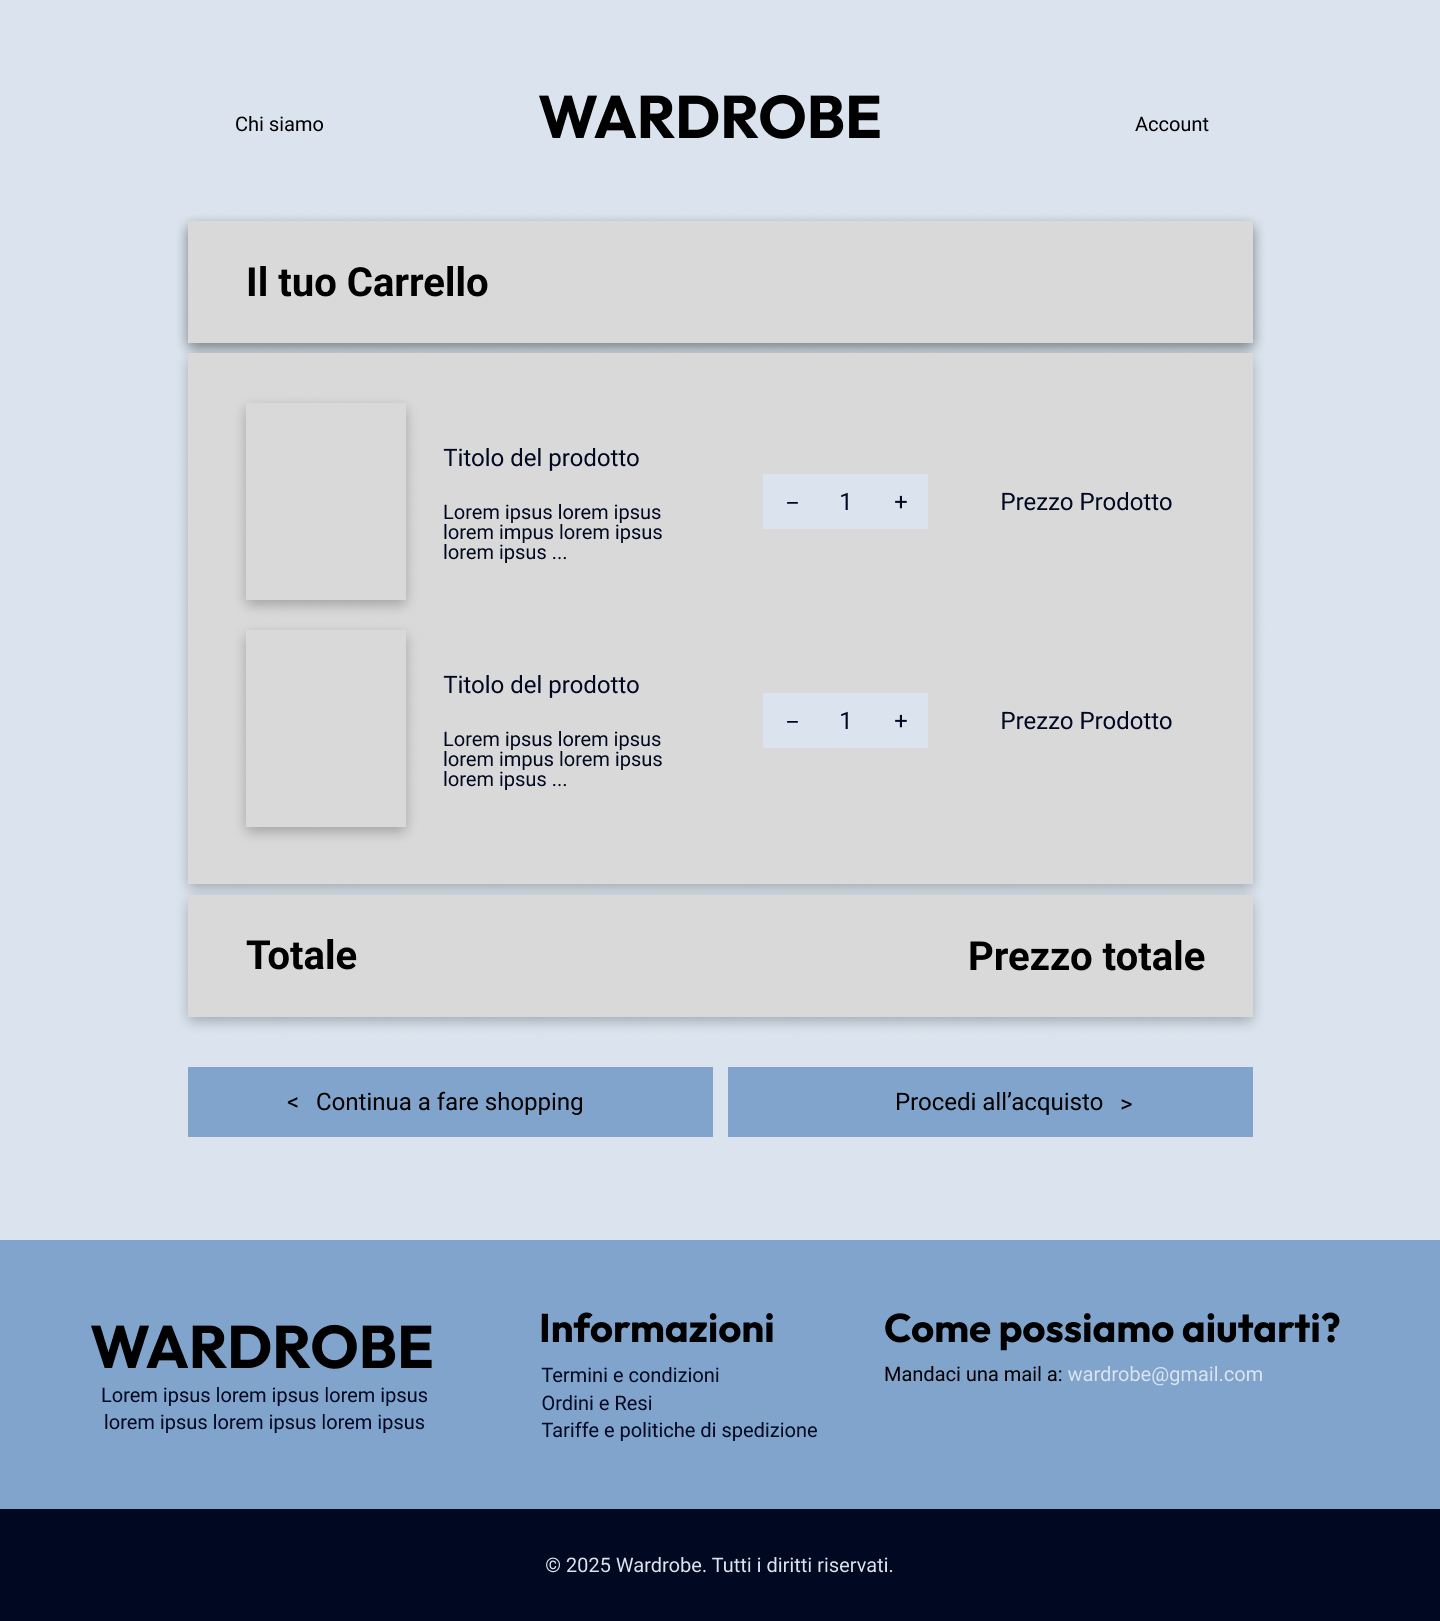
\includegraphics[width=0.8\textwidth]{immagini/Mockups/carrello.png}
\caption{Pagina del carrello}
\end{figure}

\clearpage

\begin{figure}[h!]
\centering
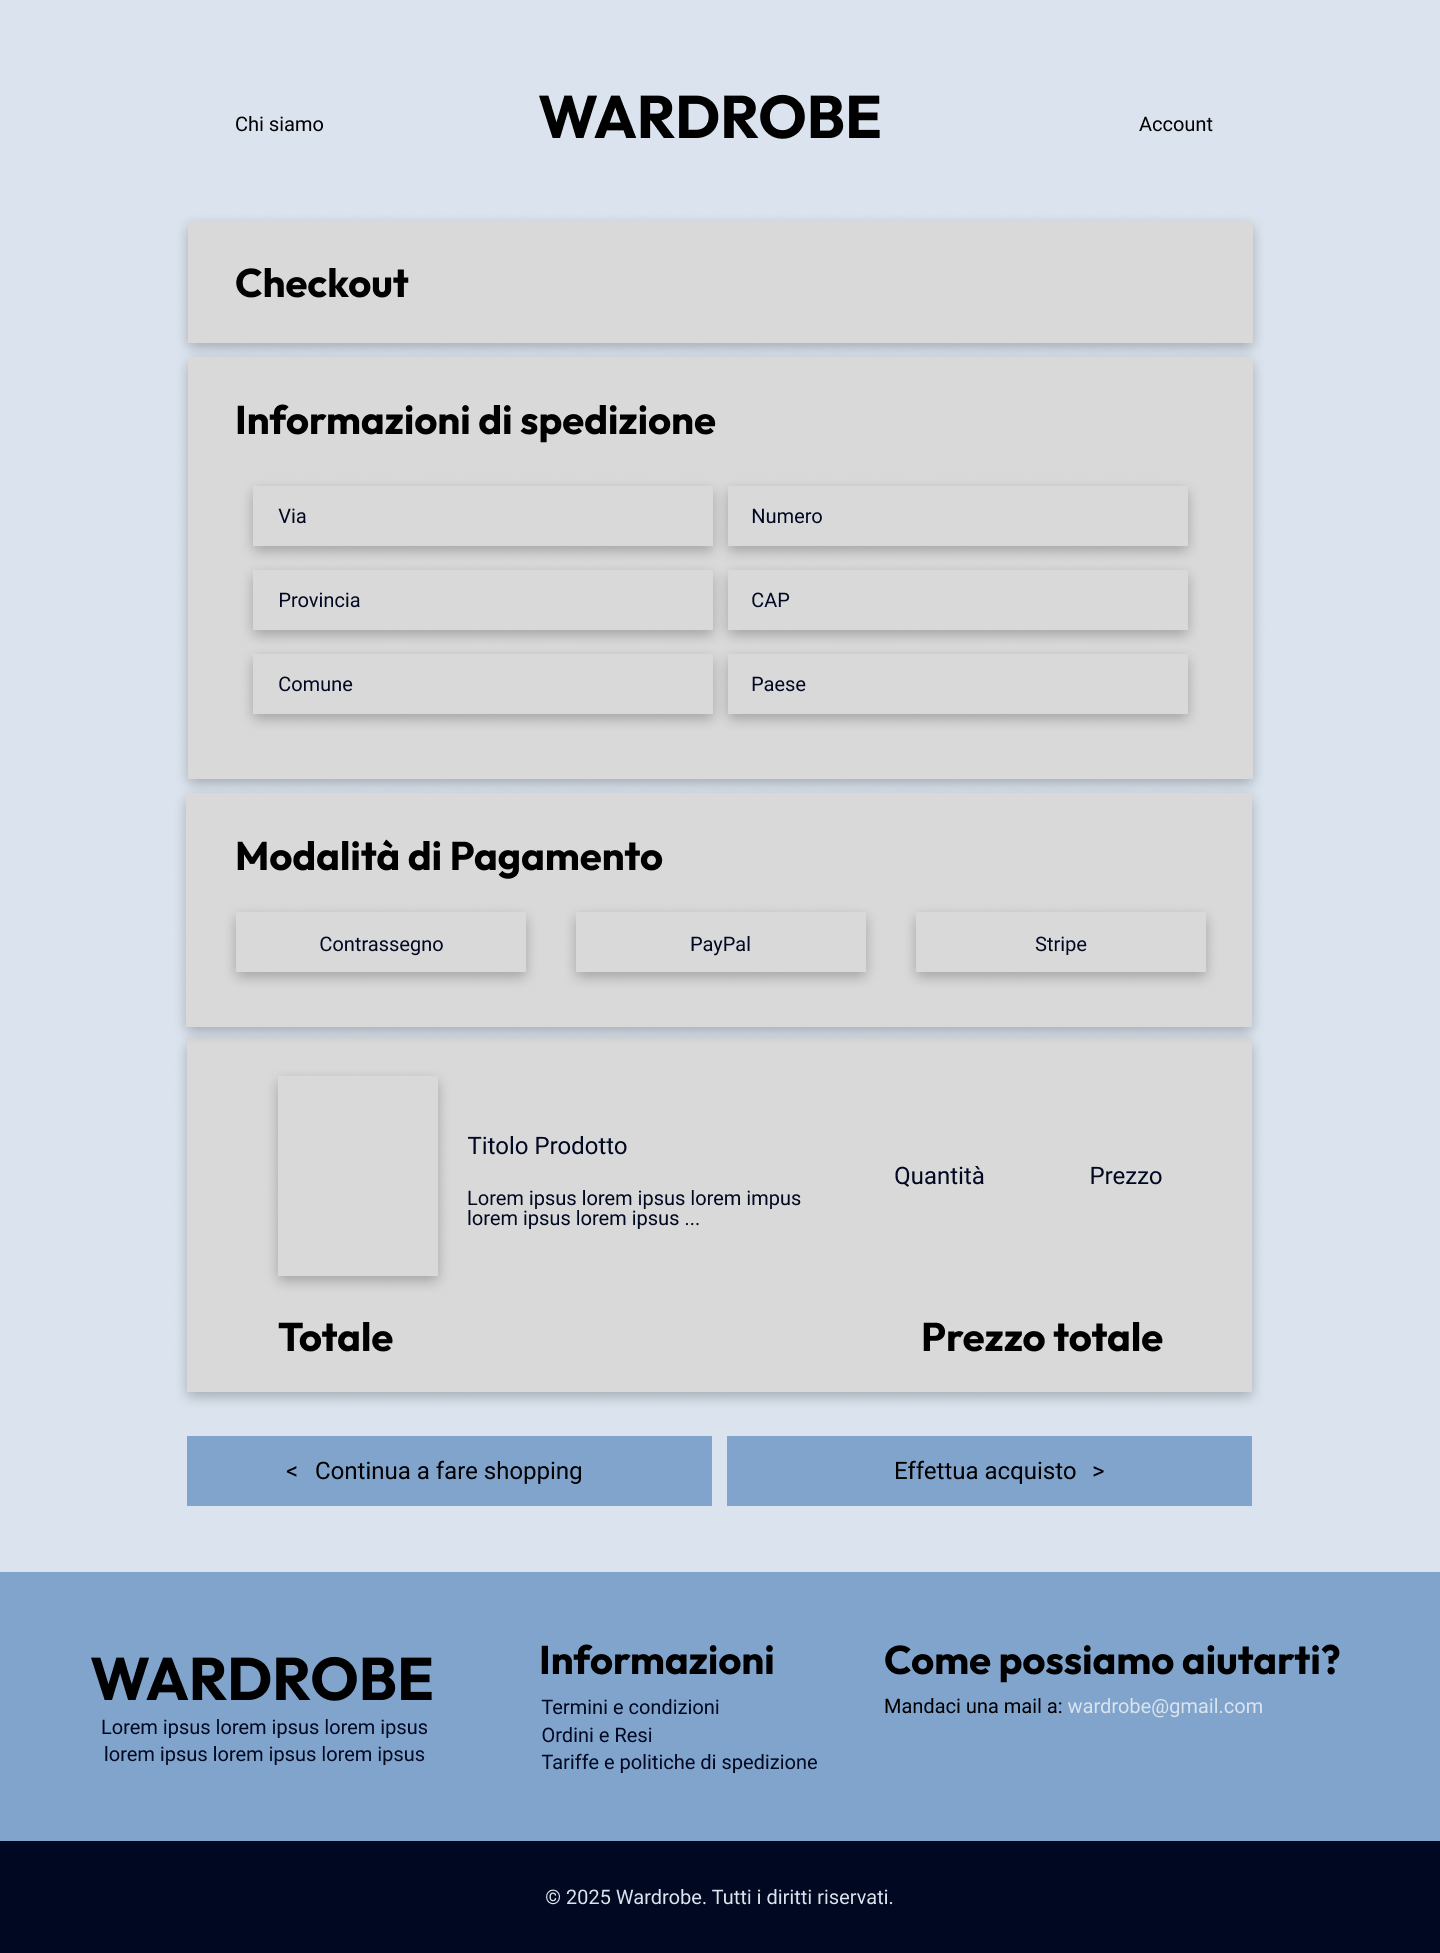
\includegraphics[width=0.8\textwidth]{immagini/Mockups/checkout.png}
\caption{Pagina di checkout dell'ordine}
\end{figure}



\clearpage
\section{Descrizione unit tests}
I seguenti test rappresentano un insieme di unit test scritti utilizzando il framework Django TestCase per garantire il corretto funzionamento di alcune classi modello di un progetto di e-commerce. Sono state testate le entità principali del sistema: "User", "Product" e "Review"; per verificare che le loro funzionalità fondamentali si comportino come previsto, contribuendo a individuare eventuali bug in fase di sviluppo.\\
\subsection{Classe ProductTestCase}
\begin{itemize}
    \item Testa gli attributi fondamentali come name, description e price.
    \item Verifica che il metodo "\_str\_" generi una rappresentazione basata su id e name.
\end{itemize}
\begin{listing}[!ht]
\begin{minted}[
frame=lines,
framesep=4mm,
baselinestretch=1.1,
bgcolor=LightGray,
fontsize=\footnotesize,
linenos
]{python}
class ProductTestCase(TestCase):
    @classmethod
    def setUpTestData(cls):
        # Set up non-modified objects used by all test methods
        Product.objects.create(name="productName",
                               price=Decimal('0.01'),
                               description="productDescription",
                               brand=Brand.objects.create(name="BrandName")
                               )

    def test_name(self):
        product = Product.objects.get(id=1)
        product_name = product.name
        self.assertEqual(product_name, 'productName')

    def test_description(self):
        product = Product.objects.get(id=1)
        product_description = product.description
        self.assertEqual(product_description, 'productDescription')

    def test_price(self):
        product = Product.objects.get(id=1)
        product_price = product.price
        self.assertEqual(product_price, Decimal('0.01'))

    def test_object_name_is_id_and_name(self):
        product = Product.objects.get(id=1)
        expected_object_name = f'{product.id}-{product.name}'
        self.assertEqual(str(product), expected_object_name)
\end{minted}
\end{listing}

\clearpage
\subsection{Classe ReviewTestCase}
\begin{itemize}
    \item Assicura che le relazioni con Product e User funzionino correttamente.
    \item Verifica gli attributi specifici come title, description e vote.
\end{itemize}
\begin{listing}[!ht]
\begin{minted}[
frame=lines,
framesep=4mm,
baselinestretch=1.1,
bgcolor=LightGray,
fontsize=\footnotesize,
linenos
]{python}
class ReviewTestCase(TestCase):
    @classmethod
    def setUpTestData(cls):
        # Set up non-modified objects used by all test methods
        Review.objects.create(
            product=Product.objects.create(
                name="productName",
                price=Decimal('0.01'),
                brand=Brand.objects.create(name="BrandName")
            ),
            user=User.objects.create(
                email='hello@world.com',
                first_name='hello',
                last_name='world'
            ),
            title="reviewTitle",
            description="reviewDescription",
            vote=1,
        )

    def test_product(self):
        review = Review.objects.get(id=1)
        product_name = review.product.name
        self.assertEqual(product_name, 'productName')

    def test_title(self):
        review = Review.objects.get(id=1)
        review_title = review.title
        self.assertEqual(review_title, 'reviewTitle')

    def test_description(self):
        review = Review.objects.get(id=1)
        review_description = review.description
        self.assertEqual(review_description, 'reviewDescription')

    def test_vote(self):
        review = Review.objects.get(id=1)
        review_vote = review.vote
        self.assertEqual(review_vote, 1)
\end{minted}
\end{listing}
\clearpage

\subsection{Classe UserTestCase}
\begin{itemize}
    \item Verifica che l'attributo email sia configurato correttamente.
    \item Controlla che il metodo "\_str\_" restituisca correttamente l'email dell'utente.
\end{itemize}
\begin{listing}[!ht]
\begin{minted}[
frame=lines,
framesep=4mm,
baselinestretch=1.1,
bgcolor=LightGray,
fontsize=\footnotesize,
linenos
]{python}
class UserTestCase(TestCase):
    @classmethod
    def setUpTestData(cls):
        # Set up non-modified objects used by all test methods
        User.objects.create(email='hello@world.com',
                            first_name='hello',
                            last_name='world'
                            )

    def test_email(self):
        user = User.objects.get(id=1)
        field_label = user.email
        self.assertEqual(field_label, 'hello@world.com')

    def test_object_name_is_email(self):
        user = User.objects.get(id=1)
        expected_object_name = f'{user.email}'
        self.assertEqual(str(user), expected_object_name)
\end{minted}
\end{listing}
